\thispagestyle{empty}

{\small
\begin{wrapfigure}{l}{2cm}
\centering
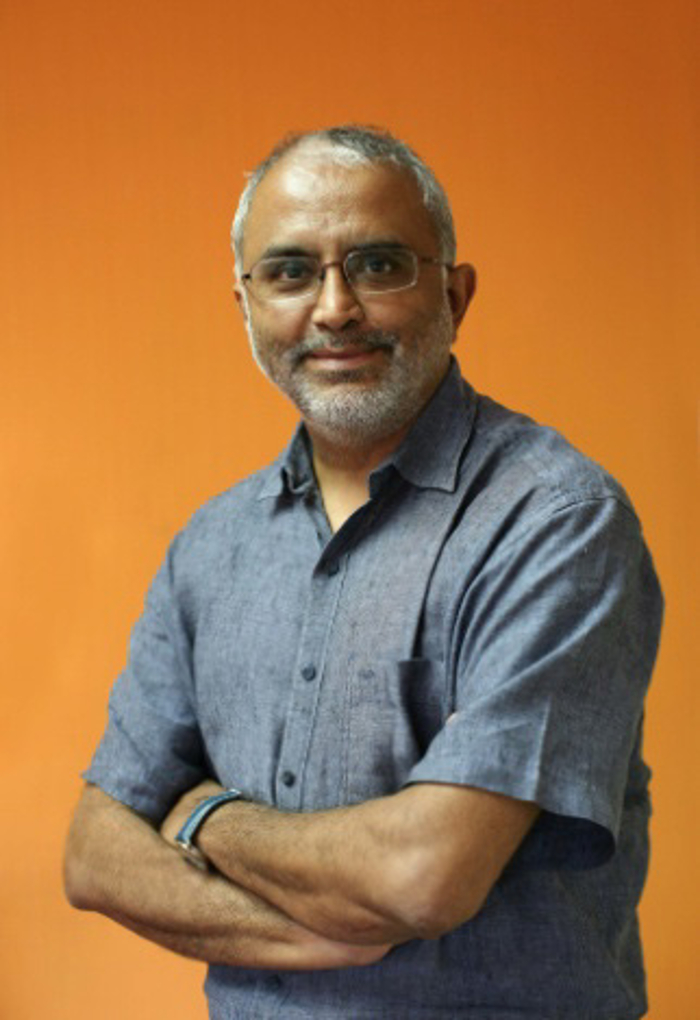
\includegraphics[scale=2.2]{images/097.jpg}
\vskip -.4cm
\end{wrapfigure}

\textcolor{maroon}{Dr. V. Lakshminarayan, acquired his MD degree from the prestigious Mysore University, and a Graduate Diplomate in Diabetes Care from The University of New Castle, Australia.}

\textcolor{maroon}{Born in a remote village into an agricultural family, he sacrificed a prestigious Faculty position at the Bangalore Medical College to go back to his rural roots and serve the underprivileged. His vision helped him identify the rising tide of diabetes in India, and he proceeded to acquire higher education in diabetes care. Since then he has been striving selflessly to educate the public about the diabetes epidemic in India through the mass media by volunteering his time on television, radio and print media. He is also caring for the sickest diabetics at his center, often times free of cost, and has earned the sobriquet “Common man’s sweet doctor”.}

\textcolor{maroon}{To raise awareness on diabetes he authored a Kannada book titled\break “Madhumeha - Dashavyadhigala Moola”, which earned the “Supreme\break Medical Literature Script” award in 2011 from P. S. Shankara Prathishttana.}

\textcolor{maroon}{In 2013, in recognition of his unparalleled efforts in serving the poor,\break especially in the field of diabetes, the Government of Karnataka awarded\break him the prestigious “Rajyotsava Award” in the field of Medicine, which is the highest recognition accorded by the State of Karnataka in 2013. In recogni\-tion of his academic works and social service, Kuvempu university conferred the degree of Doctor of Letters(Honoris Causa) in 2016. Considering the\break “Excellence of Service in the Field of Medicine” has been honoured with\break Dr. B.R.Ambedkar National Award in 2017.}

\begin{wrapfigure}{l}{2cm}
\vskip -.3cm
\centering
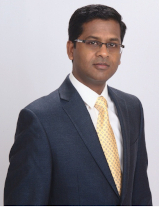
\includegraphics[scale=2.2]{images/098.jpg}
\vskip -.3cm
\end{wrapfigure}

\textcolor{maroon}{Dr. Sooraj Tejaswi is an Associate Professor and was the Director of the Gastroenterology Fellowship at the University of California Davis, one of the world’s leading research and teaching institute. He obtained his MBBS degree from the prestigious Mysore Medical College. As a recipient of the prestigious Indian Academy of Sciences research scholarship, his publications in the field of clinical diabetes research conducted at the All India Institute of Medical Sciences\break (AIIMS) has been cited more than 100 times. After this he obtained a Master’s in Public Health from the Ohio State University in USA, a postgraduation in Internal Medicine followed by a Fellowship in Gastroenterology \& Hepatology from the Cook County Hospital in Chicago. He is currently focused on health issues affecting the Indian diaspora in the United States.}

}
